% Chapter 2
\chapter{Literature Review Methodology} % Main chapter title

\label{Chapter2} % For referencing the chapter elsewhere, use \ref{Chapter1} 

Based on the guidance obtained from a previous investigation on how to conduct a literature review, the authors decided to perform a systematic analysis of the existing literature. In this process, specific protocols and techniques are clearly described so that other researchers can replicate the study and get the same results. 


A systematic literature review is one type of literature review that has a formal and structured procedure to synthesize the knowledge of existing research studies that are relevant to answer pre-defined research questions \cite{kofod-petersen_how_nodate, kitchenham_guidelines_2007}. It allows us to understand the current state of the literature and identify research gaps\cite{carrera-rivera_how-conduct_2022}. 

Additionally, we adhered to the three-phase approach to conducting a systematic literature review as outlined by Kitchenham and Charter\cite{kitchenham_guidelines_2007}, which includes planning protocol, conducting the review, and reporting results. This approach ensures that the systematic literature review is conducted in a structured and transparent manner according to Kitchenham\cite{kitchenham_guidelines_2007}. Utilizing this guideline and additional resources, we present a flow diagram of the scheme as depicted in Figure \ref{fig:slr-proc}. 

In this study, the literature review has two main objectives. First, identify existing solutions that leverage Digital Twin to enhance the security of (I)IoT applications. Secondly, to identify and investigate the security mechanism employed to secure the data which could be at rest or in transmission between the digital twin station and the data source(i.e., (I)IoT devices)


\begin{figure}[H]
    \centering
    \caption{A flow diagram of the review process.}
    \includegraphics[width=0.9\textwidth]{images/slrmethoddiagram.drawio.png}
    % \includesvg[width=1\textwidth]{images/svg/slrmethoddiagram.drawio.svg}
    
    \label{fig:slr-proc}
\end{figure}


To automate the systematic literature review process, from defining PICOC to data extraction, we use a web tool called\textit{parsif.al}\footnote{\href{https://parsif.al}{Parsifal} is an online tool designed to support researchers in performing systematic literature reviews in the context of software engineering. Geographically distributed researchers can work together within a shared workspace, designing the protocol and conducting the research}


\section{Review Protocol}
According to Kitchenham et al. \cite{kitchenham_guidelines_2007}, it is essential to define a review protocol that outlines the procedures and methods before beginning the review process. The protocol serves as a roadmap for conducting the review and ensures that the study can be replicated by providing a clear and detailed plan of the procedures to be followed\cite{carrera-rivera_how-conduct_2022}.

% \subsection{PICOC and Synonyms}
%----------------------------------------------------------------------------------------
% ======================================================================================================
% NOTES, TODOS
% ======================================================================================================

\subsection{Defining PICOC}
PICOC stands for Population, Intervention, Comparison, Output and context. It is a widely used technique in medical and social science studies to define the focus of the research\cite{carrera-rivera_how-conduct_2022}. However, in\cite{carrera-rivera_how-conduct_2022, kitchenham_guidelines_2007} Kitchenham and Carrera showed that this technique can still be applied for computer science related research to formulate and structure research questions. In this subsection, we define our PICOC criteria for this systematic literature review.

\textit{Population:} The motivation to conduct this research is the security related problem we identified in the communication between Digital Twin and constrained  (I)IoT devices deployed in the smart industry to collect sensor data. Hence, the problem domain or "Population" for this research is (I)IoT devices used with Digital Twin to enhance security in Industry 4.0. Industries that use Digital Twin and (I)IoT devices, such as smart cities, smart homes, smart grids, smart health, smart manufacturing, etc. In this sense, the "Population" part of PICOC in this review refers to the following terms: Digital Twin, (Industrial)Internet of Things, Industry 4.0, Smart Manufacturing, Cyber-physical Systems, and Critical Infrastructure. 

\textit{Intervention:} Our intervention to address this problem, the security issue of digital communication between Digital Twin and (I)IoT, is to implement a lightweight NIST standard cryptographic authentication/encryption scheme for power and computation constraint (I)IoT devices. In this regard, we use the term "authentication" as an intervention.

\textit{Comparison:} Before designing and implementing an intervention for a specific problem, it is important to identify the existing solution in the literature. The results of reviewing, comparing and analysing the existing solution discussed in the relevant research literature can be used as input to design and implement the intervention methodology. With this regard, this study will identify and compare authentication schemes or security mechanisms used in securing a data flow between Digital Twin and (I)IoT. 

\textit{Outcome:} Secure remote access with integrity and confidentiality of communication, efficient and performant cryptographic schemes that can run on constrained devices is the expected outcome of this research.\\

\textit{Context:} This systematic literature review is focused on the Industry 4.0 environment, targeting Digital Twin solutions deployed in smart industries to enhance security. However, the second part of the study is dedicated to designing and implementing authentication schemes for the Smart Grid which is considered as one instance of Industry 4.0.
%----------------------------------------------------------------------------------------


% \subsection{Research Questions}
%----------------------------------------------------------------------------------------
% ======================================================================================================
% NOTES, TODOS
% ======================================================================================================

\subsection{Research Question}
Before embarking on the process of identifying studies and extracting data, it is crucial to identify and clearly define research questions or objectives, as they serve as guiding principles for conducting a literature review\cite{carrera-rivera_how-conduct_2022}. Consequently, this systematic literature review aims to address the following research questions:

\begin{itemize}

    % RQ1
    \item \textbf{RQ1: How is Digital Twin used to enhance the security of (I)Iot applications in the industry 4.0 use cases ?} - 
    this question aims to identify how Digital Twin is used to improve the security of industries that use IoT devices, including sensors and actuators, to achieve OT (operational technology) security goals: Safety, reliability, and availability.
    % \begin{itemize}
    %     % I need a comment from Mohammed on this -> with regad to use case -> is to braod and vogue?
    %     \item \textbf{RQ1.1: What is the concrete concept of Digital Twin} - 
    %     under subcategory of the above research question, the concept of digital and its use cases are explored.
    % \end{itemize}

    % RQ 1
    % \item RQ1. What mututal authentication schemes for DT and IoT application are discussed in the literature? 
    % \item How can we use Digital Twin to enhance security issue in IoT/IIoT application? 
    %  Replace schemes by  mechansims.
    \item \textbf{RQ2: What are the security methods presented in the literature to ensure the authentication between Digital Twin and its mapped physical devices?} - 
    this question focus on the identification of authentication mechanisms that are used to ensure the security of DT and (I)IoT communication.
\end{itemize}
%----------------------------------------------------------------------------------------

% \subsection{Key Terms and Search Strategy}
%----------------------------------------------------------------------------------------
% ======================================================================================================
% NOTES, TODOS
% ======================================================================================================
% Define the search strategy for each database if possible 
% Also prepare table with or and operators refer poatek
% I need to modify the title and the resarch question -> Iot to IIoT , the area is in manufcturing or Industry 4.0.
% receive comment on the keyword variants. example IIoT, schemes.
% =======================================================================================================
\subsection{Search keys and Strategies}
Guided by the PICOC criteria and  research questions, we construct four main search strings to create search queries used for each selected databases. These are, "Digital Twin" "IoT" "Authentication", and "Industry". Synonyms, alternative spellings, and similar semantic meanings are considered for each keyword and combined using OR operator. 

During pilot search, on majority of databases, we identified adding synonyms of "Digital Twin" does not return new paper compared to searching using only the term "Digital Twin". Hence, we avoided to use other "Digital Twin" synonym terms for simplicy of our search query. 

\begin{table}[h]
% \captionsetup{
%   justification=raggedright,
%   singlelinecheck=false,
%   margin=60pt % adjust margin as needed
% }
% \centering
\caption{ Key terms and key variants.}
\begin{NiceTabular}{p{3.2cm}p{11cm}}
\toprule
    \textbf{Key terms} & \textbf{Variants / Synonyms / Similar Semantic Meaning} \\
    \midrule
    Digital Twin & DT, digital-twin, digital-twins, digital replica, digital shadow, virtual model, virtual clone \\ \hline
    (Industrial)Internet of Things & IoT, IIoT, internet-of-things, internet-of-thing, industrial internet of things, industrial-internet-of-thing, sensors, actuators, smart devices  \\ \hline
    Authentication & security, confidentiality, certificate, verification, scheme, schemes\\ \hline
    Industry & industry 4.0, manufacturing, smart manufacturing, factory, smart factory, cyber-physical system, cyber-physical systems, cyber physical systems, cyber physical system, critical infrastructure, critical infrastructures. \\ 
\bottomrule
\end{NiceTabular}
\end{table}

% As an example, an advance search query for Scopus databases is shown in table \ref{}.\\


% \begin{table}[h]
% % \centering
% \caption{\label{scopus-advanc-search} Example of advanced search query in Scopus}
% \begin{NiceTabular}{Y{1.1}}
% \CodeBefore
%   \rowcolor{gray!50}{1}
%   \rowcolors{2}{gray!25}{white}
% \Body
%  ("dt" OR "digital twin" OR "digital twins" OR "digital-twin" OR "digital-twins" OR "digital replica" OR "digital shadow" OR "virtual model" "virtual clone")  \\
%  AND \\
%  ("internet of things" OR "internet of thing" OR "internet-of-thing" OR "internet-of-things" OR "IIoT" OR "industrial internet of things" OR "industrial-internet-of-thing" OR "sensors" OR "actuators" OR "smart devices" )  \\
%  AND \\
% ("security" OR "authentication" OR "certificate" OR "verification" OR "schemes") \\
%  AND \\
% ("industry" OR "industry 4.0" OR "manufacturing" OR "smart manufacturing" OR "factory" "smart factory" OR "cyber-physical systems" OR "cyber-physical system" OR "cyber physical system")  \\
% \end{NiceTabular}
% \end{table}
%----------------------------------------------------------------------------------------

% \subsection{Digital Library}
%----------------------------------------------------------------------------------------
% ======================================================================================================
% NOTES, TODOS
% ======================================================================================================
% One paragraph about the databases 
% A table that show description and reason for selection
\subsection{Digital Library Sources}

In an attempt to perform an exhaustive search on literature that has relevant studies to our research question, we leverage six electronic archives (databases) that are known in publishing papers on computer science. These are ScienceDirect, SpringerLink, Scopus, IEEExplore, ACM, and WebofScience.  Six of them were selected in accordance with quidelines provided by Kofod \cite{kofod-petersen_how_nodate} and Kitchenham \cite{kitchenham_guidelines_2007}. 




%----------------------------------------------------------------------------------------

% \subsection{Inclusion and Exclusion Critera}
%----------------------------------------------------------------------------------------
% ======================================================================================================
% NOTES, TODOS
% ======================================================================================================

\subsection{Inclusion and Exclusion Criteria }
\label{sec:inc-exc}


\textit{Inclusion}: We only considered studies written in English, easily accessible in full text, and published in journals or conferences in the field of computer science between 2016 and 2022. 

\textit{Exclusion:} Any studies that did not meet the inclusion criteria, including those written in a language other than English, not accessible in full text, classified as gray literature, published before 2016, or not related to computer science or our research questions, were excluded from the selection process. The inclusion and exclusion criteria utilized for the purpose of filtering research studies from the search results of databases are presented in Table \ref{tbl:table-inc-exc}. 


\begin{table}[H]
\centering
\caption{\label{tbl:table-inc-exc}Inclusion and exclusion criteria.}
\begin{NiceTabular}{p{3cm}p{6cm}p{5cm}}
\toprule
    \textbf{Criteria Type} & \textbf{Inclusion} & \textbf{Exclusion} \\
    \midrule
    \textbf{Period} & Studies published between 2016 and 2022 & before 2016 \\ 
    \textbf{Language} & English & Not English \\
    \textbf{Accessibility} & accessible in full-text & Not accessible in full-text \\ 
    \textbf{Type of source} & Journal articles, conference proceedings  & Books, book chapter, \\ 
    \textbf{Type of literature} & Of type black literature & Grey literature  \\ 
    \textbf{Relevance} & Study related to computer science & Not related to computer science \\
\bottomrule
\end{NiceTabular}
\end{table}


%----------------------------------------------------------------------------------------

%----------------------------------------------------------------------------------------
% ======================================================================================================
% NOTES, TODOS
% ======================================================================================================
% describe how to perform the detail assessment
% use numeral scale 
% Are the aim of the article clearly stated?
% Is the implementation detail explained adequately 
% does the study has direct link to research question 1 and/or question 2. 
% 
\subsection{Quality Assessment Checklist}
Beside the inclusion and exclusion criteria, it is important to evaluate the quality of the research study [kitchen]. Quality assessment checklist define the detail assessment criteria for selecting paper during screening abstract and introduction of the paper. In this stage, articles that are not relevant to the research question and the objective of the study are identified and removed [kofod]. 

Below, we outline quality assessment questions as a checklist. 
\begin{itemize}
    \item \textbf{QA1:} Does the study clearly define the aim and objective of the research?
    \item \textbf{QA2:} Does the study fully explain a methodology to secure IoT/IIoT application using Digital Twin
    \item \textbf{QA3:} Does the study has direct link to research question 1 and / or question 2?
    \item \textbf{QA4:} Does the study conducted an experiment(test) to validate the hypothesis? 
    \item \textbf{QA5:} Does the study provide detail implementation of authentication scheme?
    
\end{itemize}
The quality assessment questions outlined above were evaluated using a numerical metric scoring system, with a range of 1-5, where 1 represents an irrelevant article and 5 represents a highly relevant and qualified article. The level of agreement in answering the quality checklist questions was determined through a categorical classification system, comprising of "Agree," "Somewhat Agree," "Neutral," "Somewhat Disagree," and "Disagree." These categories were assigned corresponding weight values, with "Agree" being assigned the highest weight value of 5 and "Disagree" being assigned the lowest weight value of 1. This scoring system helped to make sure that we were evaluating the research studies in a fair and consistent way, so that the studies that were most relevant and of the highest quality were selected for the review.

%----------------------------------------------------------------------------------------

% \subsection{Defining Data Extraction Form}
%----------------------------------------------------------------------------------------
% ======================================================================================================
% NOTES, TODOS
% ======================================================================================================

\subsection{Data Extraction Form}
According to Kitchenham et al.\cite{kitchenham_guidelines_2007}, a well design data extraction form is crucial for collecting information from selected primary studies to address research questions. In this study we use parsif.al web tool to design and structure data extraction form for collecting data from selected papers.  

The data extraction form is continuously evolving during the full-text review process. 

More data to be filled..... A table with data extraction from will be drawn here. 
%----------------------------------------------------------------------------------------


\section{Conducting Review}

In this study, a total of 523 articles were retrieved from online digital databases, namely ScienceDirect, SpringerLink, Scopus, IEEExplore, ACM, and Web of Science, which are known for publishing computer science-related research studies.

For all databases, we limit the search result based on the following criteria we defined in section \ref{sec:inc-exc}. To revise, we included only papers published between 2016 and 2023 from the computer science discipline, and document-type articles from journals and conferences were considered for the final search result.

Furthermore, different search queries and strategies were employed for each selected database as they have different search mechanisms. 

% \subsection{Search Queries and Search Strategy}
%----------------------------------------------------------------------------------------
% ======================================================================================================
% NOTES, TODOS
% ======================================================================================================
\subsection{Search Queries and Search Strategy}

 Each of the selected database comes with their own way of performing advance searching. The search field and filtering option are different from one database to another. Having this into consideration, we design a search strategy we called bottom down three stage searching mechanism. The detail at each stage is explained as follow. 

First we look for the main key term -- Digital twin -- on the title of the paper. The assumption behind this is that if the research main focus is digital twin it is highly likely that its title contains digital twin. Since our main objective is to understand how digital twin is used to secure IoT application on various sectors, we then narrow the previous search result by looking for security related terms such as "authentication", "security", "encryption", and "cryptography" on the abstract. In the third stage, if the number of retrieved papers is greater than 30, we further narrow the search result by tuning our search query to look for IoT and industry related terms in the full text of the research paper. 

\begin{tcolorbox}[colback=black!5!white, sharp corners=all, colframe=white!95!black]
\textbf{Web of Science}
\tcblower
("digital twin*" OR "digital-twin*") (Title) AND ( "authenticat*" OR "cryptography" OR "security" OR "encrypt*" ) (Abstract) and English (Languages) and Article or Proceeding Paper (Document Types) and Engineering or Computer Science (Research Areas)
\end{tcolorbox}

In Web of Science, "Topic"(i.e Title, keyword, and Abstract) filed is used to search for digital twin and internet of things terms. The security related terms like authentication, encryption, cryptography and encryption as well as terms related to industry are searched on all fields. From the search results of our query, document types such as book chapters, early access,and editorial are excluded. In other words, only document of type article and conference papers are selected. We run the search query over all available years which are published under category of computer science and 30 articles are returned as a result.
\begin{tcolorbox}[colback=black!5!white, sharp corners=all, colframe=white!95!black]
\textbf{Scopus}
\tcblower
( TITLE ( ( "digital twin*" OR "digital-twin*" ) ) AND TITLE-ABS-KEY ( "authenticat*" OR "cryptography" OR "security" OR "encrypt*" ) AND TITLE-ABS-KEY ( ( "industr*" OR "Industry 4.0" OR "factor*" OR "manufactur*" OR "smart manufacturing" OR "cyber-physical system*" OR "cyber physical System*" OR "infrastructure*" OR "industrial control system*" ) ) ) AND ( LIMIT-TO ( SUBJAREA , "COMP" ) OR LIMIT-TO ( SUBJAREA , "ENGI" ) ) AND ( LIMIT-TO ( DOCTYPE , "cp" ) OR LIMIT-TO ( DOCTYPE , "ar" ) ) AND ( LIMIT-TO ( SRCTYPE , "p" ) OR LIMIT-TO ( SRCTYPE , "j" ) ) AND ( LIMIT-TO ( LANGUAGE , "English" ) )
\end{tcolorbox}
We employ the same search methodology and search terms for Scopus as we do for Web of Science. We run our query string with intention to find terms in "Article title", "Abstract" and "Keywords". While document type article and conference paper are included; conference review and book chapter are excluded. Our search result returned 97 articles in total. 

\begin{tcolorbox}[colback=black!5!white, sharp corners=all, colframe=white!95!black]
\textbf{IEEExplore}
\tcblower
("Document Title":"digital twin*" OR "Document Title":"digital-twin*") AND ("Abstract":"authenticat*" OR "Abstract":"cryptography" OR "Abstract": "security" OR "Abstract":"encrypt*") \\

Filters Applied: Conferences Journals
\end{tcolorbox}
In the case IEEE, we use a different search strategy from the above two cases. while we perform search for terms  authentication and industry related on full text , the "All Metadata" field is used to perform the others search terms on title, keywords, and abstract. Articles from conferences and journals are selected and articles under category of early access and magazines are excluded. Finally, Our query resulted in 37 research studies.   

\begin{tcolorbox}[colback=black!5!white, sharp corners=all, colframe=white!95!black]
\textbf{ACM}
\tcblower
[[Title: "digital-twin*"] OR [Title: "digital twin*"]] AND [[Abstract: "security"] OR [Abstract: "authenticat*"] OR [Abstract: "encrypt*"] OR [Abstract: "cryptography"]]

\end{tcolorbox}
ACM is a bibliographic database that exclusively focuses on publishing computing literature. In ACM we run the search query within the search field of "Anywhere". And only research articles are included, and as a result 12 research studies are retrieved. 





%----------------------------------------------------------------------------------------


% \subsection{Search Result and Bibliometric Analysis}
%----------------------------------------------------------------------------------------
% ======================================================================================================
% NOTES, TODOS
% ======================================================================================================
\subsection{Search Result and Bibliometric Analysis}
Following the selection process using the inclusion and exclusion criteria, and the removal of duplicate studies, a total of 74 research papers were considered for further review and analysis. Of these, 44(60\%) were conference papers, while the remaining 40\% were journal articles.

The Majority of the selected papers were retrieved from Web of Science and Scopus, with approximately 41\% and 23\% respectively, as both are the major citation databases. Furthermore, a notable proportion of papers were also obtained from other sources, including the IEEE Digital Library (15.1\%), Springer Link (11\%), ACM Digital Library (6.8\%), and Science Direct (2.7\%). These finding are illustrated in Figure \ref{fig:archive-itemtype}, using pie chart in terms  of document type and source archive. These chart highlight the importance of leveraging a wide range of digital archives to ensure a comprehensive review of the literature. 

% \begin{figure}
% \includesvg[width=0.5\textwidth]{images/svg/databases.svg}
% \includesvg[width=0.5\textwidth]{images/svg/itemtype.svg}
% \svgcaption{This is the label for the SVG image.}
% \label{fig:image}
% \end{figure}

\begin{figure}[H]
    \centering
    \begin{subfigure}[b]{0.45\textwidth}
        % \includegraphics[width=\textwidth]{image1.png}
        \includesvg[width=\textwidth]{images/svg/databases.svg}
        \caption{Percentage of papers per database}
    \end{subfigure}
        \begin{subfigure}[b]{0.45\textwidth}
        % \includegraphics[width=\textwidth]{image2.png}
        \includesvg[width=\textwidth]{images/svg/itemtype.svg}
        \caption{Proportion of papers per item type}
    \end{subfigure}
    \caption{Paper distribution}
    \label{fig:archive-itemtype}
\end{figure}


Analysis of the distribution of selected papers based on publication year revealed that the majority of articles were published in 2022 and 2021. Furthermore, the bar chart illustrates a general upward trend in the number of publications addressing security concerns for industries utilizing Digital Twin and (I)IoT applications. This trend indicates that there is a growing interest and concern among researchers in the field of Digital Twin and IoT security, and highlights the relevance and timeliness of this systematic literature review.

\begin{figure}[H]
    \includesvg[width=0.9\textwidth]{images/svg/pub_year_white_bg.svg}
    \caption{Number of published papers per year}
    \label{fig:bar-chart-yaer}
\end{figure}
% \hajj{please remove the background color of the figure}
To gain a deeper understanding of the trending topics within the 74 selected papers published between 2018 and 2023, a frequency analysis of keywords was conducted. This analysis was performed by extracting keywords that appeared more than three times in the abstracts and keyword sections of the articles, using the VOSviewer tool. Further filtering and sensitization was applied to create a shortlist of keywords. Additionally, keywords which have similar meanings with different spellings and variations were merged. The resulting frequency analysis of keywords, illustrated in Figure \ref{fig:alluvial-key}, provides valuable insights into the key themes and concepts that are prevalent in current research on the topic of Digital Twin and IoT security. This analysis can help guide future research by identifying areas where there is a need for further investigation and providing a sense of the current state of the field.


\begin{figure}[H]
    % \includesvg[width=0.9\textwidth]{images/svg/key_buble.svg}
    % 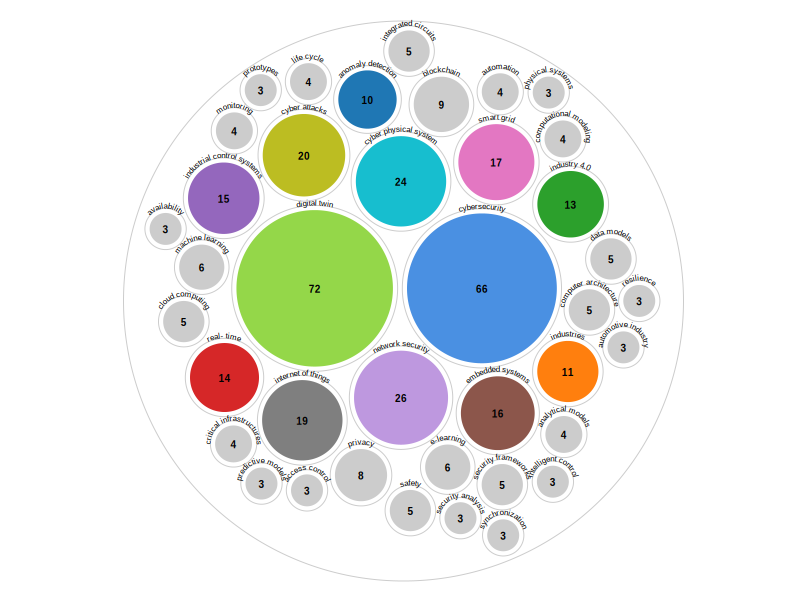
\includegraphics[width=\textwidth]{images/svg/key_buble.png}
    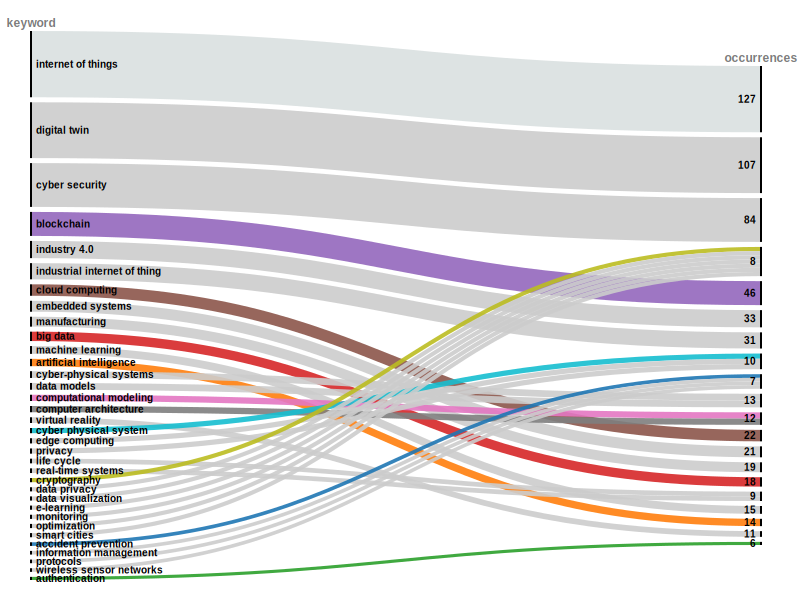
\includegraphics[width=\textwidth]{images/key_belt.png}
    \caption{Frequency of keywords}
    \label{fig:alluvial-key}
\end{figure}

Bibliographic information from 175 papers is used to generate 1187 keywords. Using thesaurus text file, we configure the tool to merge keywords that have similar semantic meaning. Moreover, we set a minimum threshold to limit the result to 87 keywords that meet 3 occurrences of the 1187 keywords.    


The analyisis of the selected papers using VOSviewer software revealed that which terms were frequently mentioned on the abstract and keyword section of the paper. The most frequently mentioned terms were "digital twin" with 72 occurrences, followed by "cybersecurity" with 66 occurrences, "cyberphysical system" with 24 occurrences, "cyber attacks" with 20 occurrences, "internet of things" with 19 occurrences, and "embedded systems" with 17 occurrences.This analysis highlights the key themes and concepts that are prevalent in current research on the topic of Digital Twin and IoT security. The high frequency of the term "digital twin" indicates the centrality of this concept in the field and the importance of understanding its role in ensuring the security of industries utilizing DT and IoT applications. The frequent mention of terms such as "cybersecurity" and "cyber attacks" further emphasizes the need for robust security measures to protect these systems from malicious actors.Additionally, the presence of terms such as "cyberphysical system" and "embedded systems" highlights the need for interdisciplinary research and collaboration between experts in fields such as computer science, engineering, and physics to effectively address the security challenges facing Digital Twin and IoT.

In order to gain further insights into the evolution of research in the field of Digital Twin and IoT security, a keyword co-relationship network analysis was extracted from VOSviewer tool. This analysis aimed to identify clusters of related items and to visualize the relationships between keywords over time. The results of this analysis revealed that in the early days of research on Digital Twin, keywords such as "monitoring", "safety", "prototypes", "resilience", "software", and "tools" were frequently mentioned, which suggests that the primary focus of research at that time was on utilizing Digital Twin as a visual aid. However, more recent research is characterized by the frequent mention of emerging technologies such as "blockchain," "machine learning," "e-learning" "5G," and "privacy" This indicates that the development of Digital Twin has shifted towards utilizing these technologies to enhance its security capabilities. This highlights the importance of continuous monitoring of the research field and to adapt to new technologies and approaches for Digital Twin security.



\begin{figure}[H]
    % \centering
    % \includegraphics[width=1.5\textwidth, center]{images/vos_key_cooc_6_final.png}
    \includesvg[width=\textwidth]{images/svg/vos_co_time_2.svg}
    % \includesvg[inkscapelatex=false,width=0.95\columnwidth]{images/key_belt.svg}
    \caption{keyword co-relationship from VOSviewer}
    \label{fig:co-occurrence-vosv}
\end{figure}

The analysis of the co-occurrence of keywords in the selected articles, as represented in Figure \ref{fig:co-occurrence-vosv}, reveals the identification of five clusters. These clusters, as defined by the VOSviewer documentation, are groups of terms that exhibit a high degree of relatedness. Cluster one encompasses terms related to 5G technology, machine learning, real-time security analysis, security frameworks, access control, and automation. Cluster two comprises of keywords such as cybersecurity, data models, digital twin, internet of things, privacy, prototypes, safety, and cloud computing. The third cluster encompasses terms such as those related to the automotive industry, availability, blockchain, industry 4.0, industrial control systems, system life cycle, intelligent control, software, and tools. The fourth cluster is comprised of analytical models, anomaly detection, cyber-attacks, monitoring, resilience, critical infrastructure, integrated circuits, and physical systems. The final cluster includes terms such as cyber-physical systems, e-learning, embedded systems, predictive models, and smart grids.
%----------------------------------------------------------------------------------------

% \subsection{Study Selection and Refinement}
%----------------------------------------------------------------------------------------
% ======================================================================================================
% NOTES, TODOS
% ======================================================================================================
\subsection{Study Selection and Refinement}
% 74 selected papers -> 14 not relevant and 3 duplicate studies submitted to different journals  excluded during full review of the papers. 

Even thought, we initially selected 73 papers for analysis. Upon further examination, we discovered three studies that were duplicates with different metadata but had similar content, and had been submitted to different journals. These duplicates were not identified by the tools we had used to exclude them. In addition, through quality assessment checklist, we also excluded fourteen papers for data extraction phase.

The reasons for the exclusion of these papers were as follows:

\begin{itemize}
    \item When the paper discussed how to secure the digital twin itself, rather than securing IoT applications using digital twin technology or securing the communication channel between DT and (I)IoT. 
    \item If the paper lacked a clear objective and aim.
    \item Some were not related to securing (I)IoT applications with an Industry 4.0 use case (for example, a study that used a digital twin to secure a data centre).
    \item Study sourced from book chapter. 
    \item The study was not relevant to any of the research questions.
    \item A study that focuses on securing (I)IoT devices that are not associated with any industry use case. 
\end{itemize}

As a result of this refinement and selection process, we were left with final set of 56 papers that were used for data extraction and analysis. In the following chapter, we provide a review of the 56 papers focusing to answer two research questions: How is digital twin used to improve the security of (I)IoT applications and what security mechanisms are used to secure the communication channel?    




%----------------------------------------------------------------------------------------

% \subsection{Data Extraction and Monitoring}
%----------------------------------------------------------------------------------------
% ======================================================================================================
% NOTES, TODOS
% ======================================================================================================
\subsection{Data Extraction and Monitoring}
%----------------------------------------------------------------------------------------

% \subsection{Data Synthesis}
%----------------------------------------------------------------------------------------
% ======================================================================================================
% NOTES, TODOS
% ======================================================================================================
\subsection{Data Synthesis}
%----------------------------------------------------------------------------------------







%----------------------------------------------------------------------------------------

% Todo: Method for data extraction and synthesis 
% \subsection{Data Extraction Method}
% \subsection{Data Synthesis Method}